\documentclass{beamer}
\usepackage{graphicx}
\usepackage{url}
\usepackage[style=ieee]{biblatex}
\usepackage[T1]{fontenc} 
\usepackage{verbatim}
\setbeamertemplate{bibliography item}{\insertbiblabel}
\usecolortheme{dolphin}

\usepackage{filecontents}
% \begin{filecontents*}{mlir.bib}
%  @misc{lattner2020mlir,
%    title={MLIR: A Compiler Infrastructure for the End of Moore's Law},
%    author={Chris Lattner and Mehdi Amini and Uday Bondhugula and Albert Cohen and Andy Davis and Jacques Pienaar and River Riddle and Tatiana Shpeisman and Nicolas Vasilache and Oleksandr Zinenko},
%    year={2020},
%    eprint={2002.11054},
%    archivePrefix={arXiv},
%    primaryClass={cs.PL}
%  }
%  @misc{mlirtutorial,
%    title={MLIR Tutorial: Building a Compiler with MLIR},
%    author={Mehdi Amini and Alex Zinenko and Nicholas Vasilache},
%    year={2020},
%    howpublished="\url{https://llvm.org/devmtg/2019-04/slides/Tutorial-AminiVasilacheZinenko-MLIR.pdf}"
%  }
% \end{filecontents*}
\addbibresource{mlir.bib}

\title{MLIR - Multi-Level Intermediate Representation}
\author{Kevin Jude Concessao}
\institute{IIT Palakkad}
\date{\today}

\begin{document}

\begin{frame}
  \titlepage
\end{frame}

\begin{frame}
  \frametitle{Outline}
  \tableofcontents
\end{frame}

\section{Introduction}
\begin{frame}
  \frametitle{Introduction}
  \begin{columns}
    \begin{column}{0.6\textwidth}
      \begin{figure}[h]
        \centering
        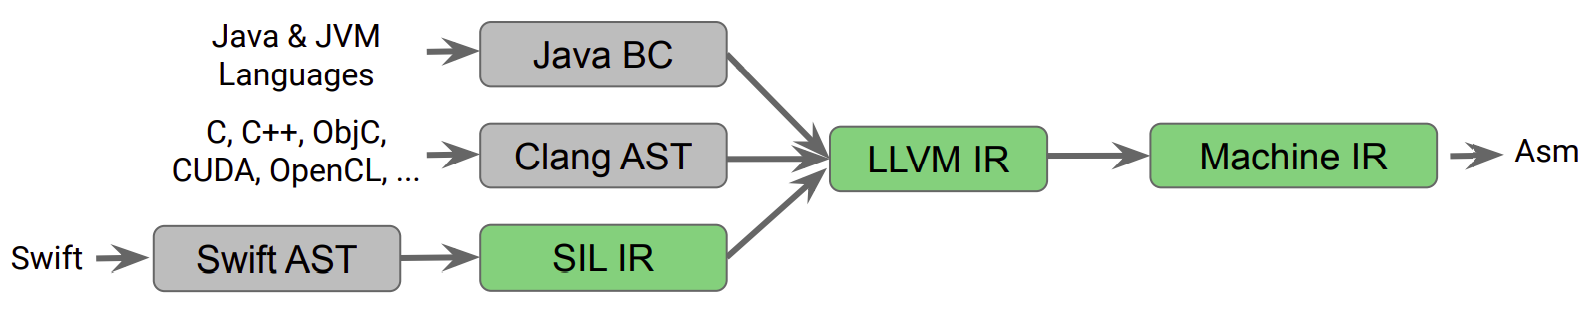
\includegraphics[width=\textwidth]{pictures/Introduction.png}
      \end{figure}
      \begin{figure}[h]
        \centering
        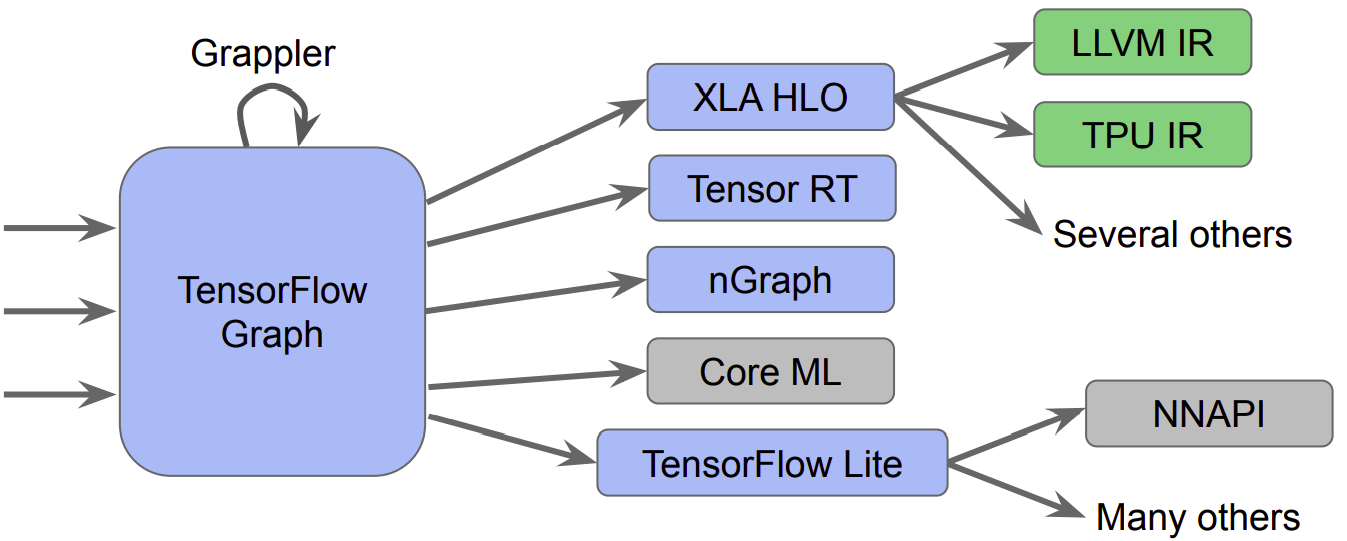
\includegraphics[width=\textwidth]{pictures/IR2.png}
      \end{figure}
    \end{column}
    \begin{column}{0.6\textwidth}
      \footnotesize
      \begin{itemize}
        \footnotesize
        \itemsep0.4em
        \item Domain specific optimizations:
          \begin{itemize}
            \footnotesize
            \itemsep0.4em
            \item Devirtualization
            \item Reference Count elision
            \item Progressive lowering
            \item Library specific optimizations
            \item Better type / borrow checking            
          \end{itemize}
        \item Problems:
        \begin{itemize}
          \footnotesize
          \itemsep0.4em
          \item Reimplementation of pass managers, error tracking, passes, use-def chains, etc.
          \item Huge expense to rebuild / repeat existing infrastructure. Wasteful repetition of effort.          
        \end{itemize}
      \end{itemize}
    \end{column}
  \end{columns}
\end{frame}

\subsection{What is MLIR ?}
\begin{frame}
  \frametitle{Introduction - What is MLIR ?}
  \begin{columns}
    \begin{column}{0.5\textwidth}
      \begin{figure}[h]
        \centering
        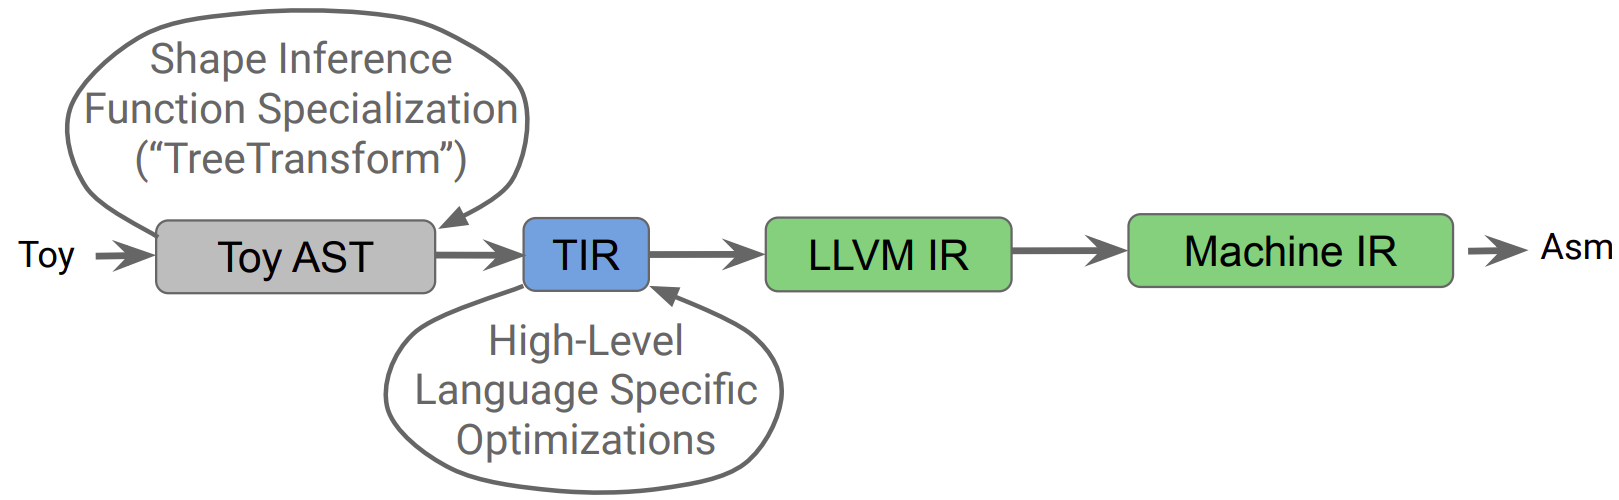
\includegraphics[width=\textwidth]{pictures/toyir.png}
      \end{figure}
    \end{column}
    \vrule
    \begin{column}{0.5\textwidth}
      \begin{figure}[h]
        \centering
        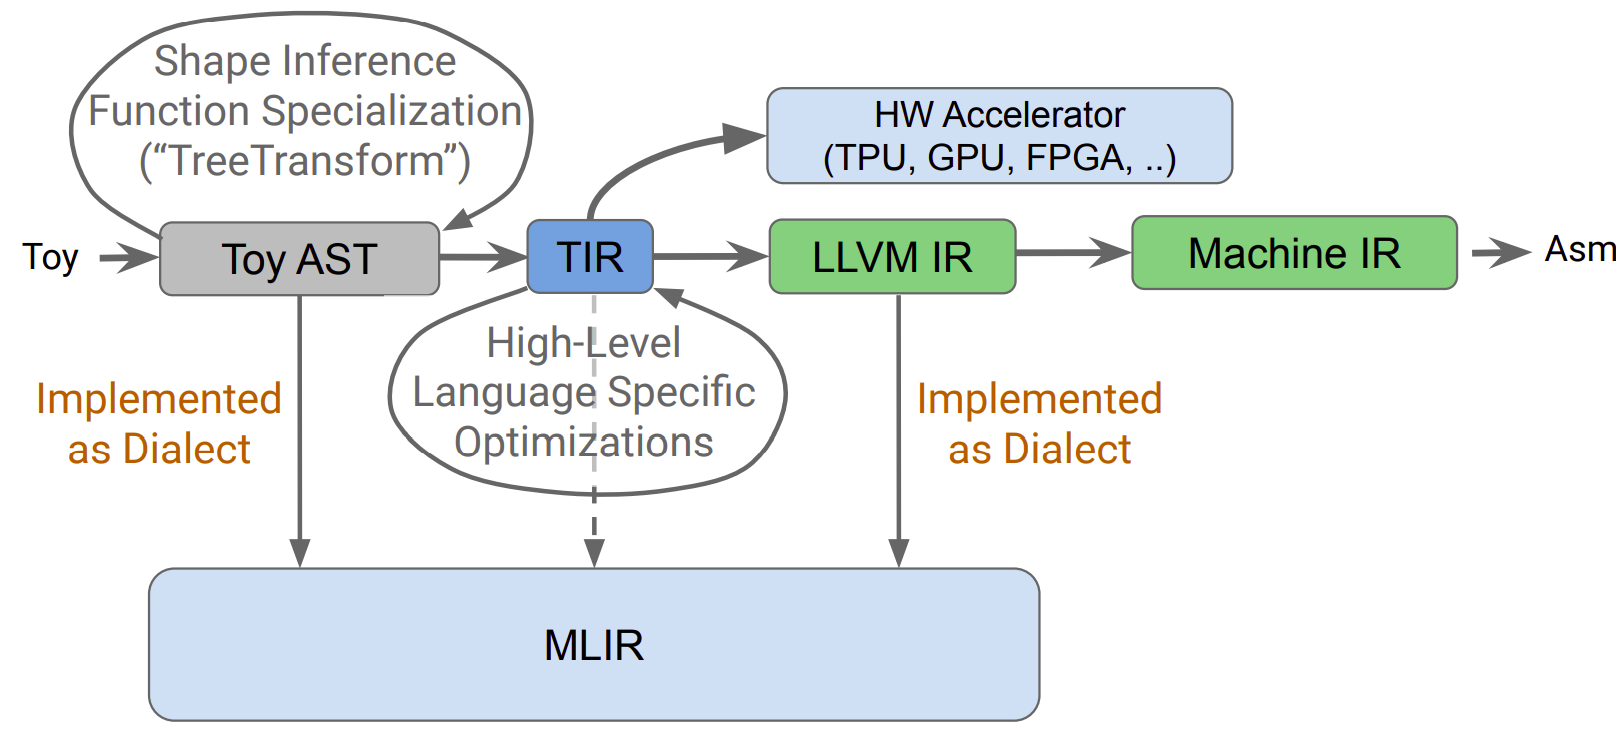
\includegraphics[width=\textwidth]{pictures/toymlir.png}
      \end{figure}
    \end{column}
  \end{columns}
  \vspace{0.5cm}
  \footnotesize
  \begin{itemize}
    \footnotesize
    \itemsep0.4em 
    \item MLIR is a \textbf{framework} to represent \textbf{multiple levels} of \texttt{tree-based} IRs, \texttt{machine level} IRs, \texttt{graph-based} IRs
    \item Provides \textbf{common infrastructure} to write \texttt{optimization}, \texttt{lowering}, and \texttt{reuse} of \textbf{pass}es across IRs.
    \item Reduces duplication of \texttt{pass infrastructure}, \texttt{location tracking / error handling}.
    \item Provides \textbf{minimal abstractions} for representing constructs across domains: \texttt{parallel constructs}, \texttt{polyhedral models}, 
    \texttt{ML graph} optimizations, etc.
    \item Not opinionated. Extensible because of minimal abstractions.
  \end{itemize}
\end{frame}

\section{Design Principles}
\begin{frame}
  \footnotesize
  \frametitle{Design Principles}
  \begin{itemize}
    \itemsep0.5em
    \item Little builtin, everything customizable
      \begin{itemize}
        \footnotesize
        \itemsep0.5em
        \item Minimal number of fundamental concepts: attributes, types, operations.
        \item Ability to express ML graphs, ASTs, polyhedral models, CFGs, LLVM IR, etc
        \item Create reusable abstractions
      \end{itemize}
    \item SSA and regions
      \begin{itemize}
        \footnotesize
        \itemsep0.5em
        \item Makes data-flow analysis simple. Well understood representation.
        \item Unlike flat-linearized CFGs, there are nested regions. lift higher level abstractions (e.g., loop trees),
        speeding up the compilation process or extracting instruction, or SIMD parallelism. 
        \item To support heterogeneous compilation, the system has to support the expression of structured control
        flow, concurrency constructs, closures in source languages, and many other purposes.
        \item Loss of normalization: lowering to a minimal subset as in LLVM. 
      \end{itemize}
  \end{itemize}
\end{frame}

\begin{frame}
  \footnotesize
  \frametitle{Design Principles}
  \begin{itemize}
    \itemsep0.5em
    \item Progressive lowering 
      \begin{itemize}
        \footnotesize
        \itemsep0.5em
        \item Benefits of combining passes was to mix constant propagation, value numbering and unreachable code elimination across dialects.
        \item Passes are meant for optimizing, transforming, lowering and cleaning dialect operations.
      \end{itemize}
    \item Maintain higher-level semantics: Only lower a construct when not need for further optimization.
    \item IR validation
    \item Declarative rewrite patterns
      \begin{itemize}
        \footnotesize
        \itemsep0.5em
        \item Common transformations should be implementable as rewrite rules expressed declaratively, to reason 
              about properties of the rewrites such as complexity and completion.
        \item Build machine descriptions capable of
        steering rewriting strategies through multiple levels of abstraction
      \end{itemize}
    \item Source location tracking and traceability
  \end{itemize}
\end{frame}

\section{IR Design}
\subsection{IR Structure - Operations}
\begin{frame}
  \frametitle{IR Design}
  \begin{itemize}
    \item Operations in MLIR are analogous to \texttt{Instruction}'s in \texttt{LLVM IR}.
    \item Operations take and produce zero or more values, called operands and results respectively, and
    these are maintained in \texttt{SSA form}.
  \end{itemize}
  \begin{figure}[h]
    \centering
    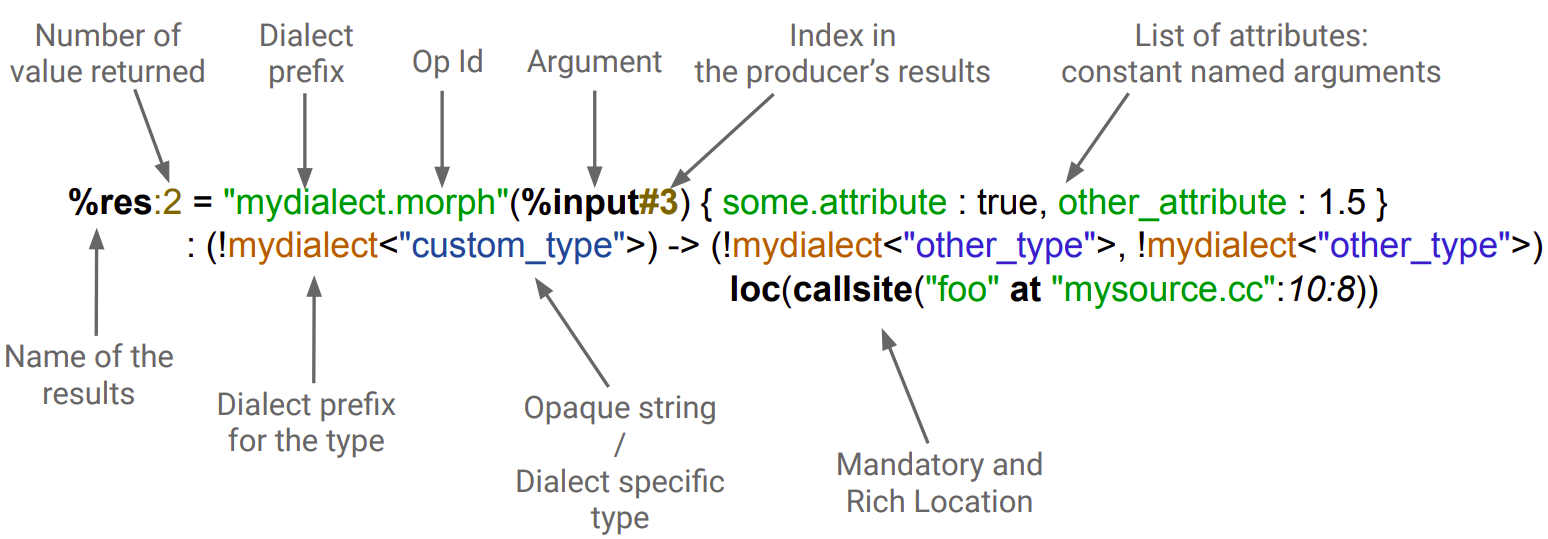
\includegraphics[width=\textwidth]{pictures/Operation.png}
  \end{figure}
\end{frame}

\begin{frame}
  \frametitle{IR Design - Nesting of Operations - Regions}
  \begin{figure}[h]
    \centering
    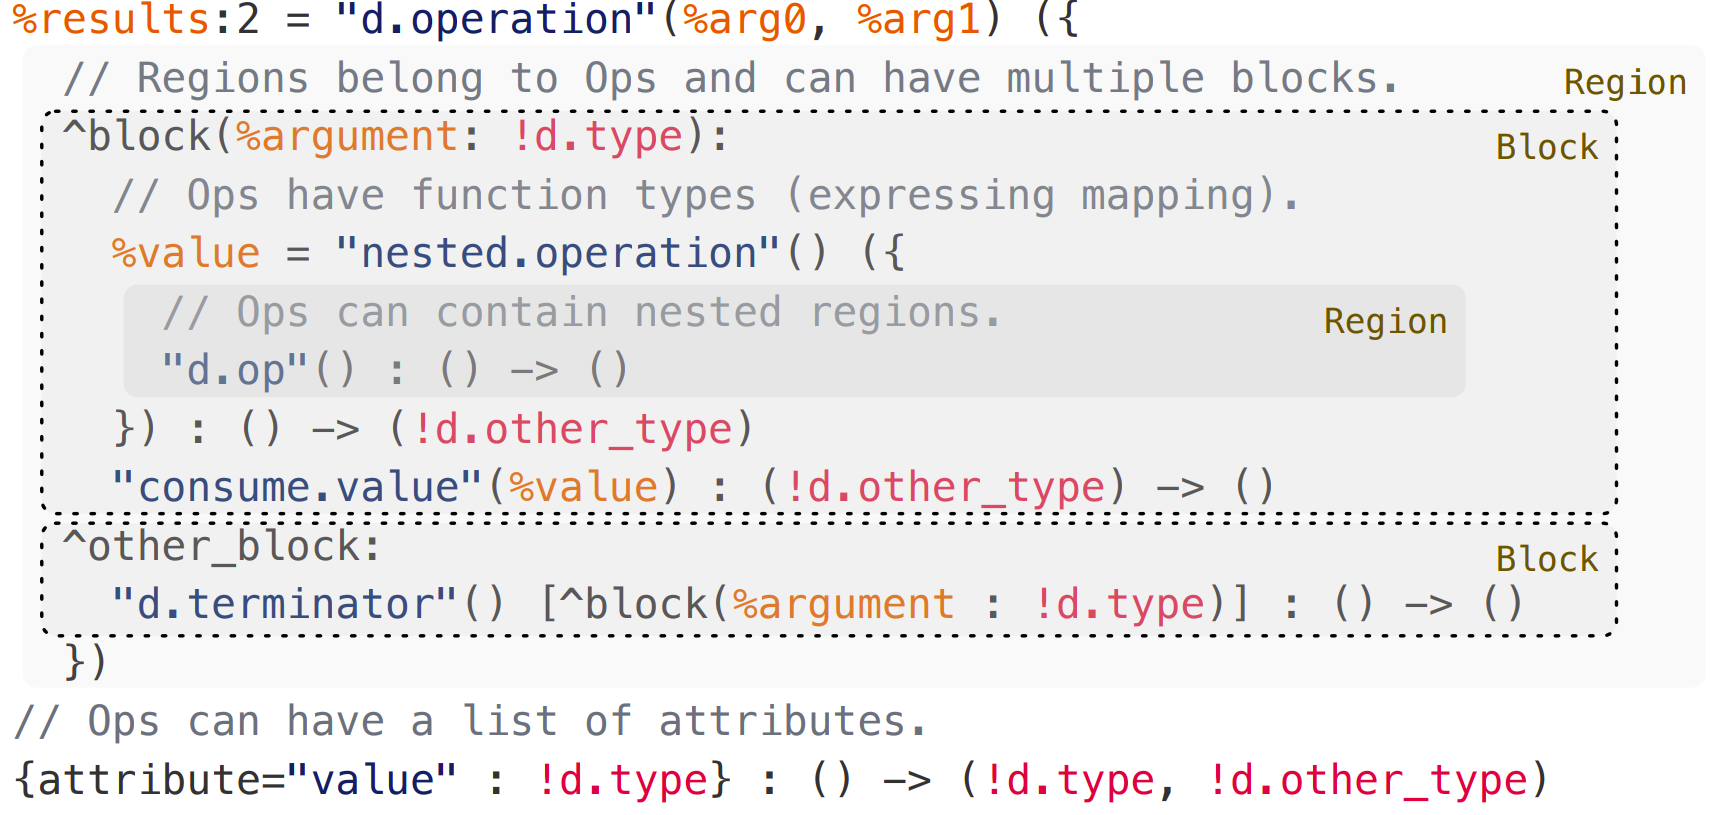
\includegraphics[width=0.8\textwidth]{pictures/BlockRegionOperation.png}
  \end{figure}
  \begin{itemize}
    \item A \textbf{region} contains a list of blocks, and a \textbf{block} contains a list of \textbf{operations} (which may contain regions).
    \item \textbf{Blocks} inside a region form a \textbf{CFG}. Each block ends with a \textbf{terminator operation}.
    \item No $\phi$ nodes. MLIR uses a \textbf{functional SSA}.
  \end{itemize}
\end{frame}

\subsection{What is a Dialect}
\begin{frame}
  \frametitle{What is a Dialect ?}
  A dialect encapsulates the following: 
  \begin{itemize}
    \item A \textbf{prefix / namespace}.
    \item A collection of \textbf{types}.
    \item \textbf{Operations}:
      \begin{itemize}
        \item Verifier for operation invariants (e.g. toy.print must have a single operand)
        \item Semantics (has-no-side-effects, constant-folding, CSE-allowed, et cetra)
      \end{itemize}
    \item \textbf{Passes}: analysis, transformations, and dialect conversions.
    \item Custom parsers and pretty-printers.
  \end{itemize}
  \vspace{0.5cm}
  Each of the above can be implemented using a \texttt{C++ class}, or with a \texttt{TableGen DSL} program for MLIR. \\ 
  \vspace{0.5cm}
  \texttt{mlir-tablegen} can auto-generate these \texttt{C++ classes}. The paper calls it as \textbf{\texttt{Operation Definition Specification}}.
\end{frame}

\subsection{Affine Dialect Example}
\begin{frame}
  \frametitle{Affine Dialect Example}
  \begin{figure}[h]
    \centering    
    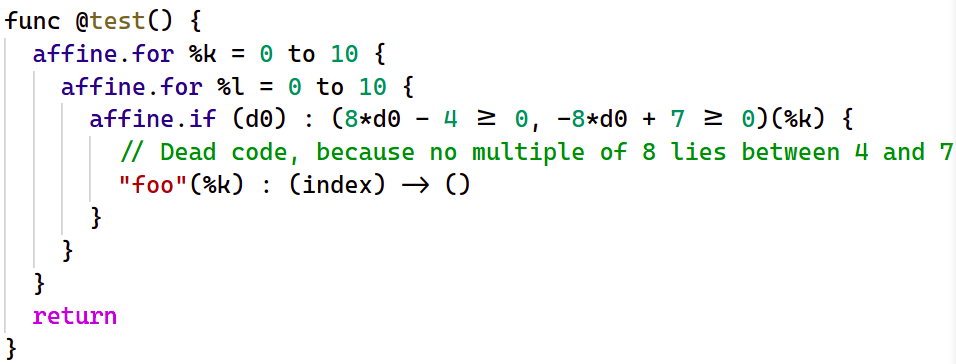
\includegraphics[width=\textwidth]{pictures/affine.png}
  \end{figure}
\end{frame}

\begin{frame}
  \frametitle{Affine Dialect Example}
  \begin{figure}[h]
    \centering
    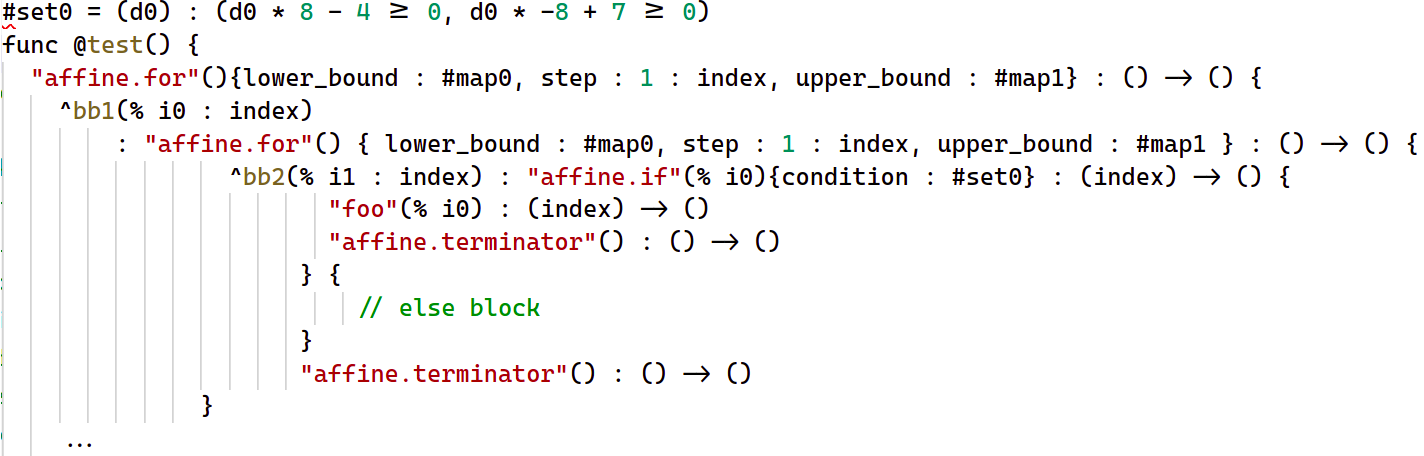
\includegraphics[width=\textwidth]{pictures/affine1.png}
  \end{figure}
\end{frame}

\subsection{LLVM Dialect Example}
\begin{frame}
  \frametitle{LLVM Dialect Example}
  \begin{figure}[h]
    \centering    
    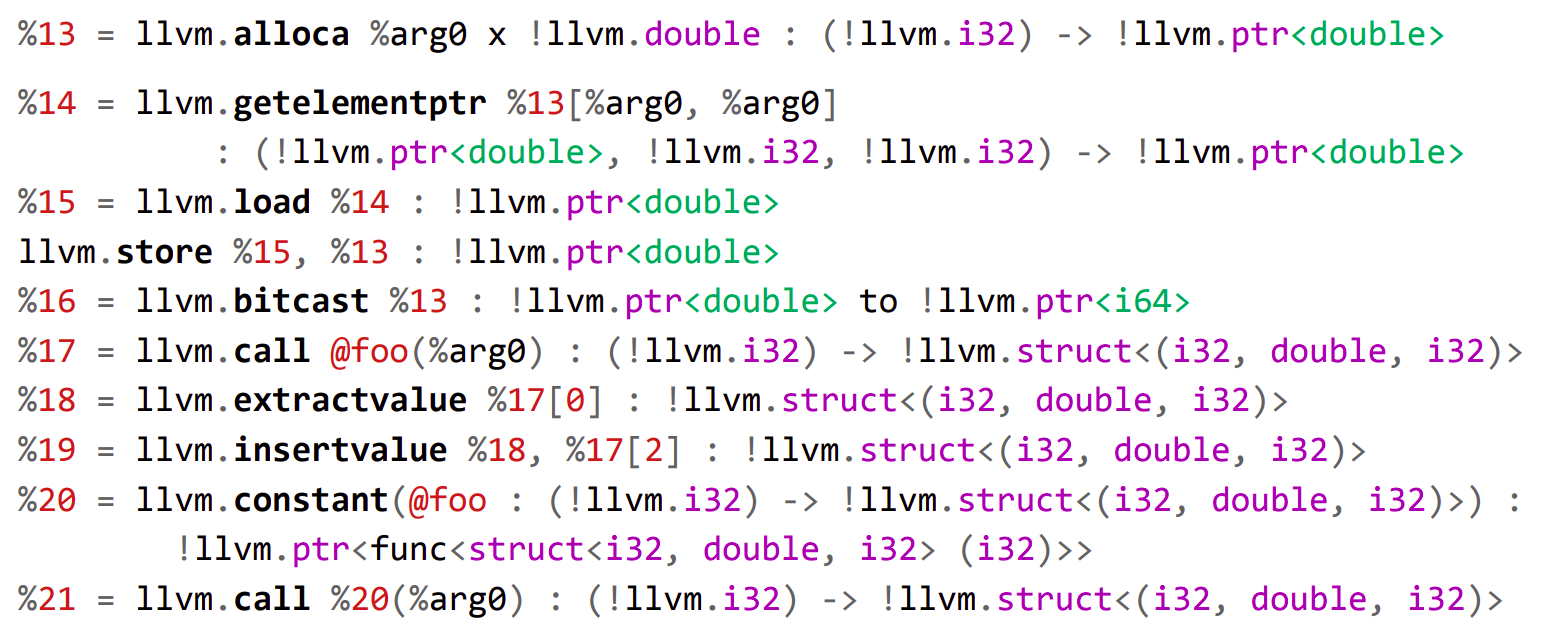
\includegraphics[width=\textwidth]{pictures/llvmdialect.png}
  \end{figure}
\end{frame}

\subsection{Operation Definition Specification}
\begin{frame}
  \frametitle{Operation Definition Specification}
  \begin{columns}
    \begin{column}{0.6\textwidth}
      \begin{figure}[h]
        \raggedright
        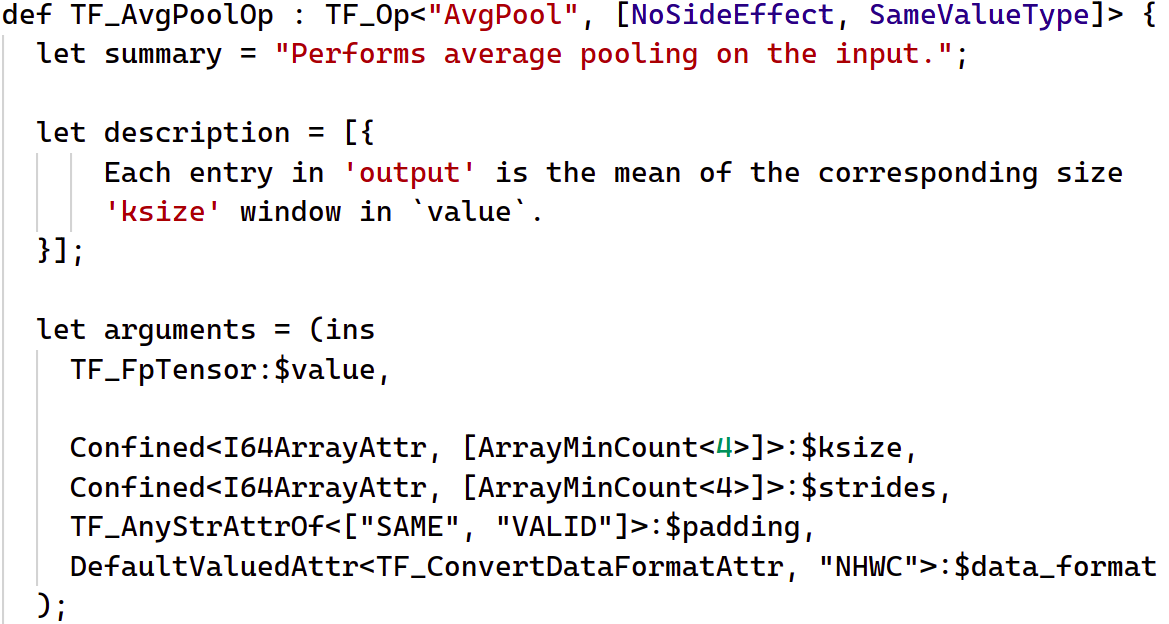
\includegraphics[width=\textwidth]{pictures/Op1.png}
      \end{figure}
    \end{column}
    \begin{column}{0.4\textwidth}
      \begin{figure}[h]
        \raggedright
        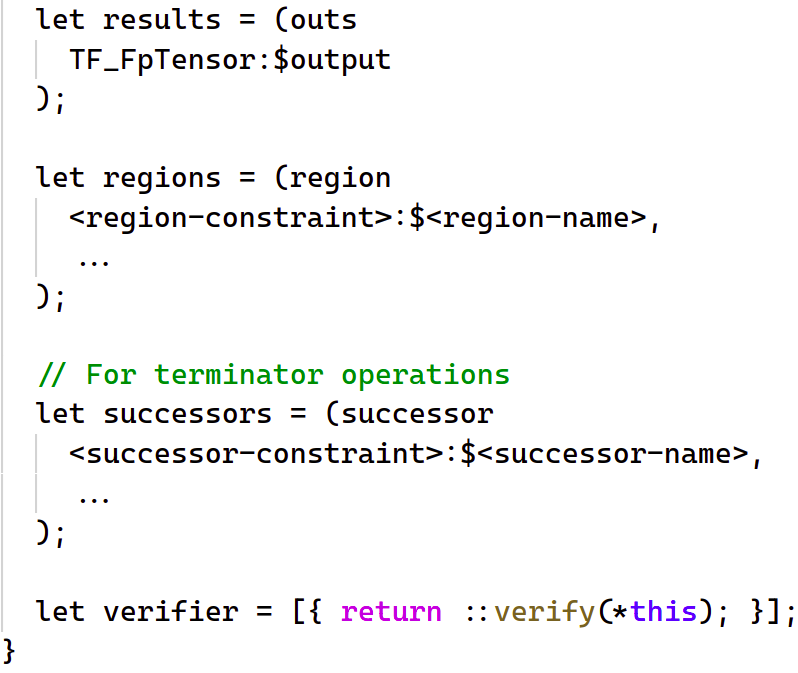
\includegraphics[width=\textwidth]{pictures/Op2.png}
      \end{figure}
    \end{column}
  \end{columns}
\end{frame}

\section{Optimization using MLIR}
\begin{frame}
  \frametitle{Optimization using MLIR}
  \begin{columns}
    \begin{column}{0.35\textwidth}
      \begin{figure}[h]
        \centering
        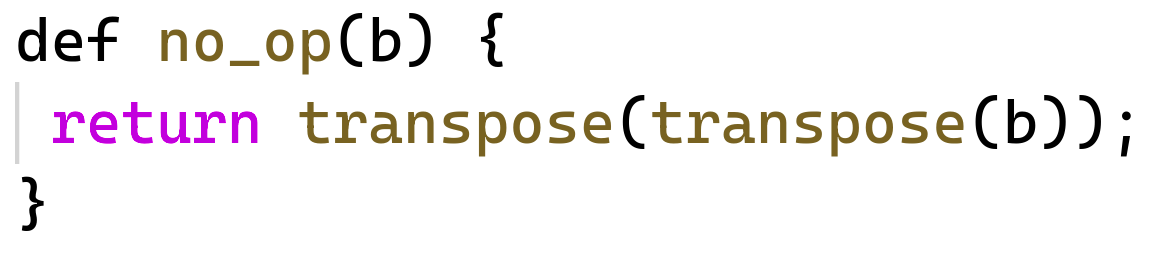
\includegraphics[width=\textwidth]{pictures/TransposeTranspose.png}
        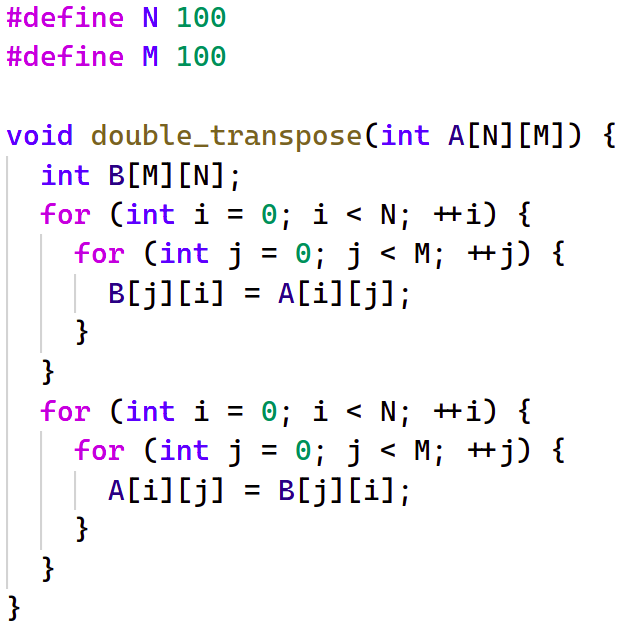
\includegraphics[width=\textwidth]{pictures/CodeExample.png}
      \end{figure}
    \end{column}
    \vrule
    \begin{column}{0.6\textwidth}
      \begin{figure}[h]
        \centering
        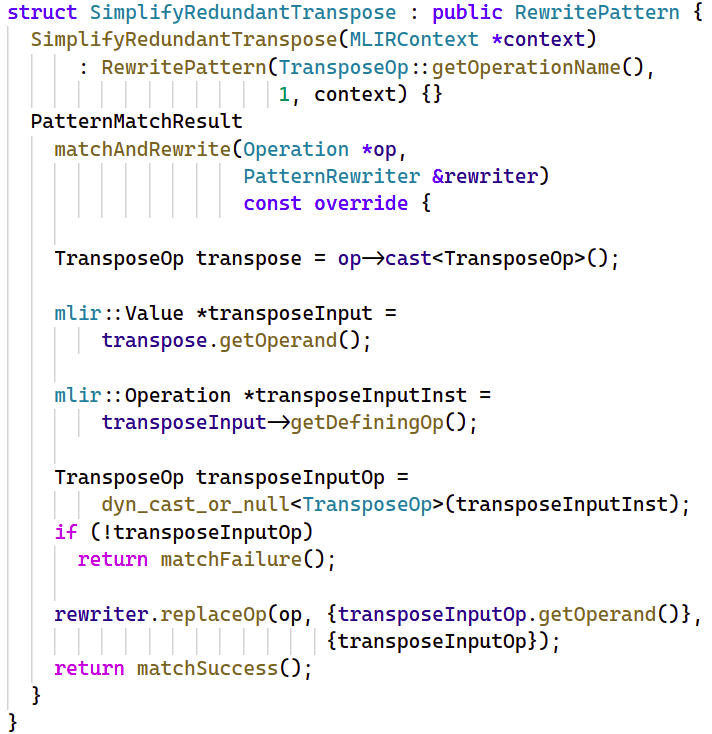
\includegraphics[width=0.9\textwidth]{pictures/PatternRewrite1.png}
        \vspace{0.1cm}
        \vspace{0.1cm}
        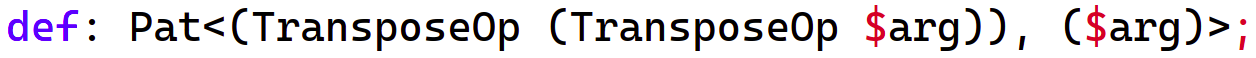
\includegraphics[width=0.9\textwidth]{pictures/TransposeTransposeOp2.png}
      \end{figure}
    \end{column}
  \end{columns}
\end{frame}

\begin{frame}
  \frametitle{Optimization using MLIR}
  Before:
  \begin{figure}[h]
    \raggedright
    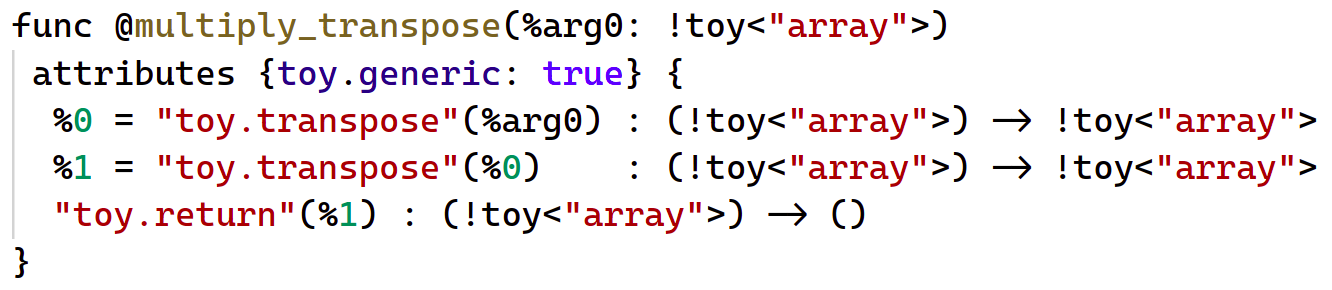
\includegraphics[width=0.9\textwidth]{pictures/BeforeOpt.png}
  \end{figure}
  After:
  \begin{figure}[h]
    \raggedright
    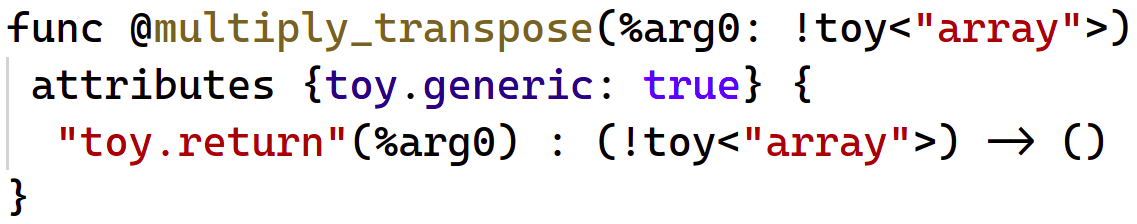
\includegraphics[width=0.65\textwidth]{pictures/AfterOpt.png}
  \end{figure}
\end{frame}

\section{Dialect Conversion}
\begin{frame}
  \frametitle{Dialect Conversion}
  \begin{columns}
    \begin{column}{0.5\textwidth}
      \begin{figure}[h]
        \centering
        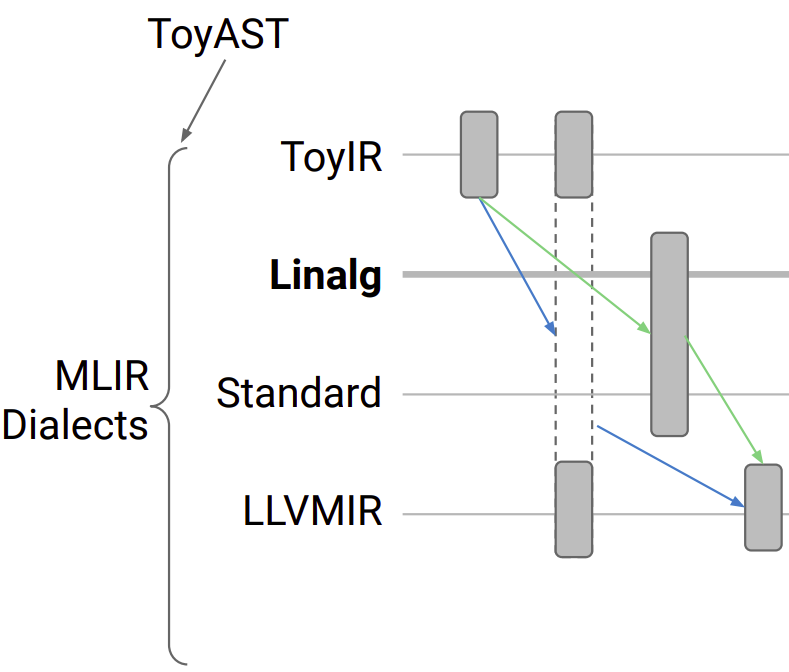
\includegraphics[width=0.9\textwidth]{pictures/DialectConversions.png}
      \end{figure}
    \end{column}
    \begin{column}{0.5\textwidth}
      {\scriptsize
        Toy Dialect: 
        \begin{itemize}
          \item \texttt{toy.constant}
          \item \texttt{toy.reshape}
          \item \texttt{toy.cast}
          \item \texttt{toy.transpose}
          \item \texttt{toy.mul}
          \item \texttt{toy.generic\_call}
          \item \texttt{toy.print}
          \item \texttt{toy.return}
        \end{itemize}
        \vspace{0.4cm}
        Standard Dialect:
        \begin{itemize}
          \item \texttt{std.br   (BranchOp)}
          \item \texttt{std.mulf (MulFOp)}
          \item \texttt{std.addi (AddIOp)}
          \item \texttt{std.cmpf (CmpFOp)}
          \item \texttt{std.xor  (XOROp)}
          \item \texttt{std.switch (SwitchOp)}
          \item \texttt{std.return (ReturnOp)}
        \end{itemize}
      }
    \end{column}
  \end{columns}
\end{frame}

\begin{frame}
  \frametitle{Dialect Conversion}
  \begin{columns}
    \begin{column}{0.5\textwidth}
      \begin{figure}[h]
        \centering
        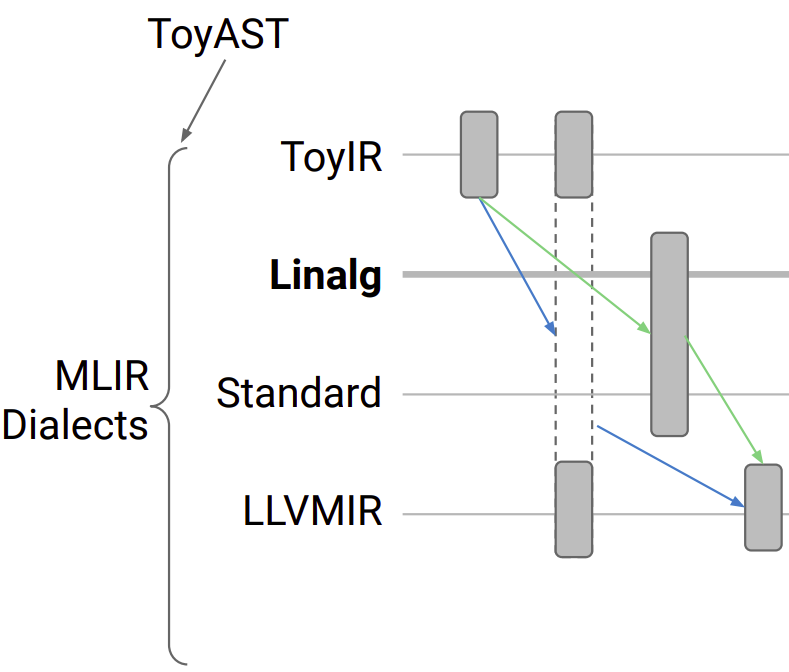
\includegraphics[width=0.9\textwidth]{pictures/DialectConversions.png}
      \end{figure}
    \end{column}
    \begin{column}{0.5\textwidth}
      {
        Linalg Dialect: 
        \vspace{0.2cm}
        \begin{itemize}
          \item Types:
            {\scriptsize
              \begin{itemize}
                \itemsep0.4em
                \item \texttt{linalg.range}
                \item \texttt{linalg.view}
              \end{itemize}
            }
          \vspace{0.2cm}
          \item Operations:
            {\scriptsize
              \begin{itemize}
                \itemsep0.4em 
                \item \texttt{linalg.matmul}
                \item \texttt{linalg.matvec}
                \item \texttt{linalg.dot}
                \item \texttt{linalg.load}
                \item \texttt{linalg.store}
                \item \texttt{linalg.range}
                \item \texttt{linalg.slice}
                \item \texttt{linalg.view}
              \end{itemize}
            }
        \end{itemize}
      }
    \end{column}
  \end{columns}
\end{frame}

\begin{frame}
  \frametitle{Dialect Conversion}
  \begin{itemize}
    \itemsep0.5em
    \item \texttt{MLIR} allows for \textbf{progressive lowering}: allows multiple dialects in the same function or module.
    \item Three components:
      \begin{itemize}
        \itemsep0.5em
        \item \textbf{Function signature} conversion
        \begin{figure}[h]
          \raggedright
          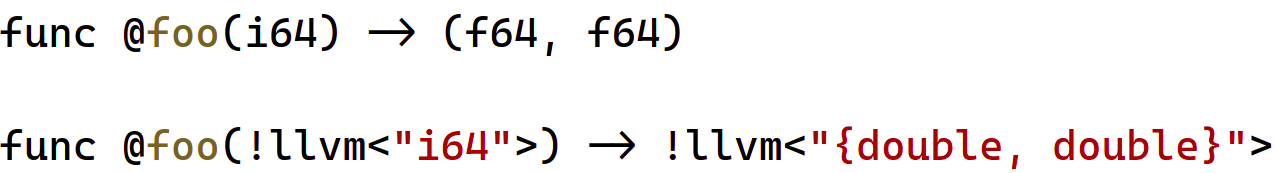
\includegraphics[scale=0.15]{pictures/signature.png}
        \end{figure}
        \item \textbf{Type} conversion
        \begin{figure}[h]
          \raggedright
          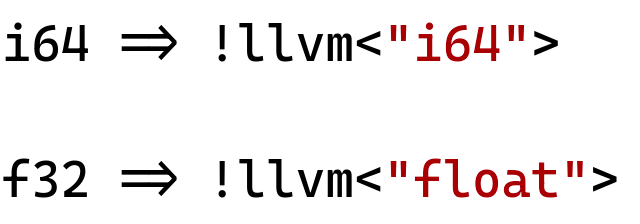
\includegraphics[scale=0.1]{pictures/typeconversion.png}
        \end{figure}
        \item \textbf{Operation} conversion
        \begin{figure}[h]
          \raggedright
          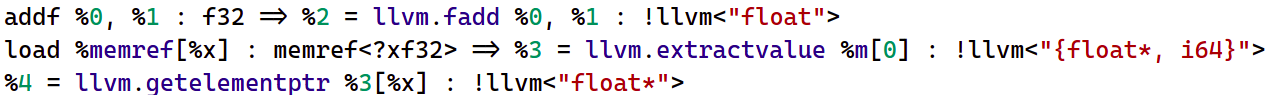
\includegraphics[width=0.9\textwidth]{pictures/operationconversion.png}
        \end{figure}
      \end{itemize}
  \end{itemize}
\end{frame}

\begin{frame}{}
  \centering
  \textcolor{purple}{\textbf{Thank You}}
\end{frame}

\nocite{*}

\begin{frame}
  \frametitle{References}
  \printbibliography
\end{frame}

\end{document}